\question Alice and Bob are throwing baseballs and they want to see who can throw a baseball further. The distance Alice throws a baseball is modeled as a uniform distribution between $0$ and $5$ while the distance Bob throws a baseball is modeled as a uniform distribution between $0$ and $10$. 
\begin{enumerate}[label=(\alph*)]
\item Assuming Alice and Bob throw independently, what is the probability that Bob's throw will be further than Alice's?
\begin{solution}[1cm]
	Let $A \mathtt{\sim} U[0, 5]$ be the distance of Alice's throw and let \\
	$B \mathtt{\sim} U[0, 10]$ be the distance of Bob's throw.  \\
	We know the density of $A$ is $\frac{1}{5}$ and the density of $B$ is $\frac{1}{10}$ \\
	We can draw the following graph where $x$ is Alice's throw and $y$ is Bob's throw. \\
	
	\begin{center}
		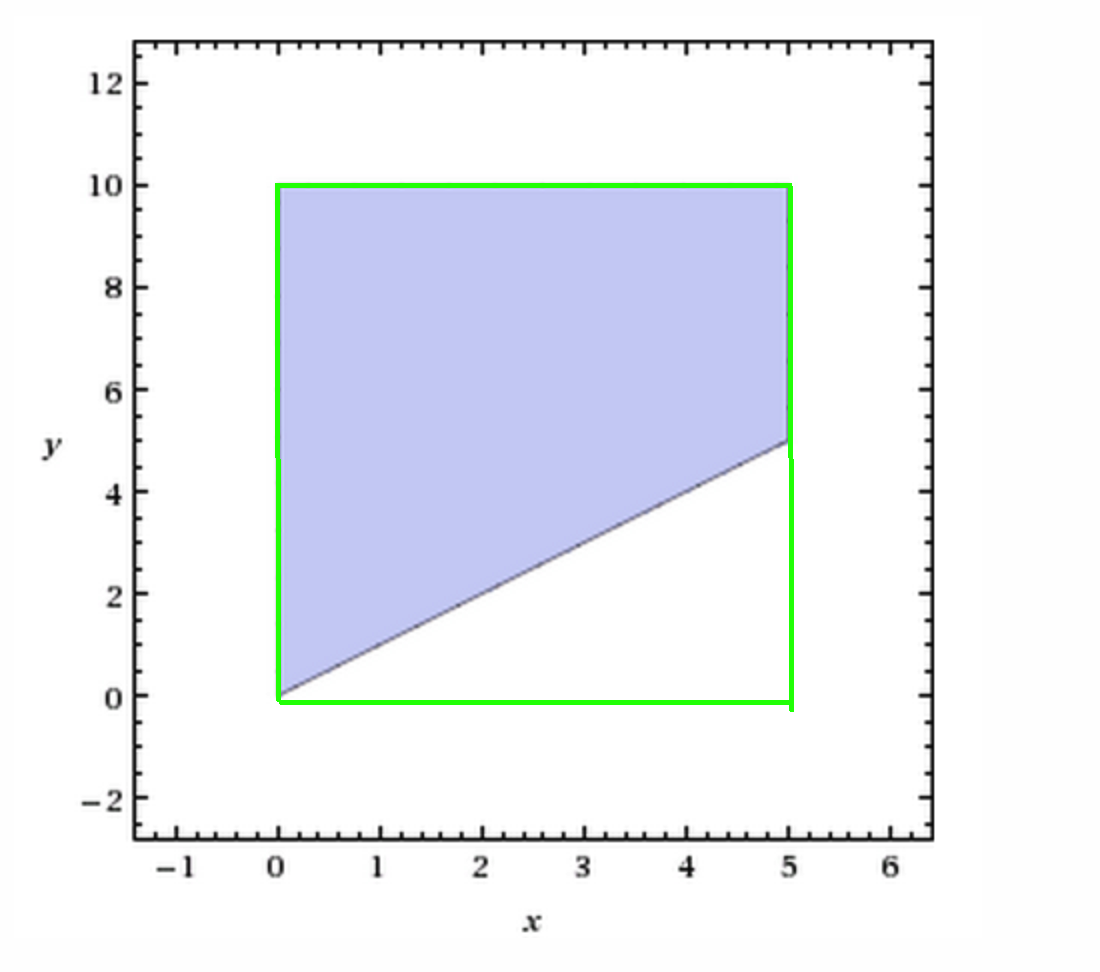
\includegraphics[width=5cm]{joint_uniform.png}
	\end{center}
	The green outline is the entire sample space while the shaded region is the region of interest. As we can see, the blue region takes up $\frac{3}{4}$ of the total sample space. \\
	
	A more algebraic approach is to use double integrals. \\
	We fix Alice's throw to be between $0$ and $5$ and we only consider Bob's throw if it is greater than Alice's. \\
	The joint pdf $f_{A, B} = f_A * f_B = \frac{1}{50}$ as $A$ and $B$ are independent.  \\
	Therefore, \\
	$P(B > A)   \\
	= \int\limits_{0}^{5}\int\limits_{a}^{10}f_{A, B} db da \\
	=  \int\limits_{0}^{5}\int\limits_{a}^{10}\frac{1}{50} db da \\
	= \int\limits_{0}^{5} (\frac{1}{50}b)\big|_{a}^{10} da \\
	=  \int\limits_{0}^{5} \frac{1}{5} - \frac{a}{50} da \\
	= (\frac{1}{5}a - \frac{a^2}{100})\big|_{0}^{5} = 1 - \frac{25}{100} = \frac{3}{4}$
\end{solution}

\item Now Alice has improved her throwing abilities and her throwing distance is now also uniform on the interval $0$ to $10$, which is the same as Bob. \\
Given that Alice's throw was greater than $5$, what is the probability that Bob throws further than her? 
\begin{solution} [1cm]
	Let $A \mathtt{\sim} U[0, 10]$ be the distance of Alice's throw and let $B \mathtt{\sim} U[0, 10]$ be the distance of Bob's throw.  \\
	We know the density of $A$ is $\frac{1}{10}$ and the density of $B$ is $\frac{1}{10}$ \\
	We want $P(B > A | A > 5)$ \\
	We can draw the following graph where $x$ is Alice's throw and $y$ is Bob's throw. \\
	\begin{center}
		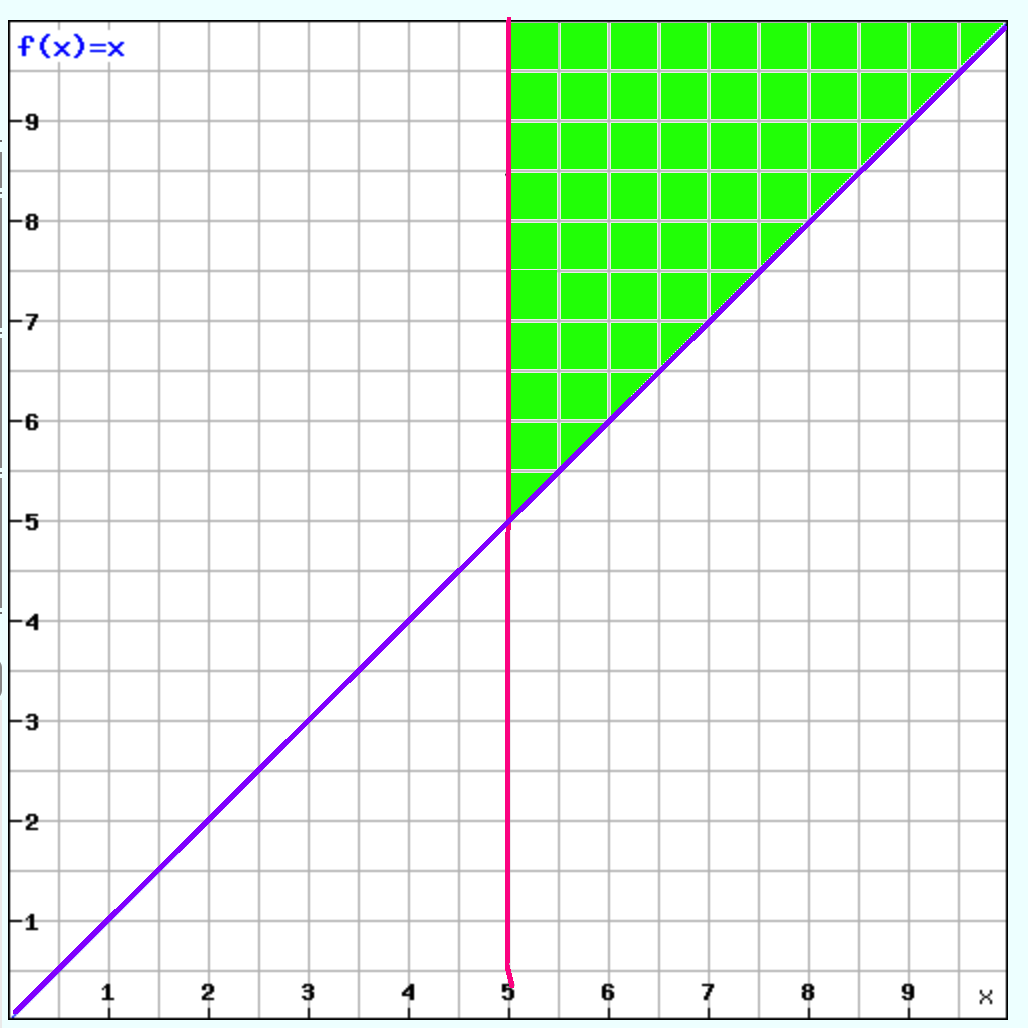
\includegraphics[width=5cm]{joint_uniform2.png}
	\end{center}
	Here let the y-axis be Bob's throw and let the x-axis be Alice's throw. \\
	Here, the purple line represents the region in which Bob throws further than Alice. \\
	The red line down the middle represents the fact that Alice's throw was greater than $5$, so we focus our attention on everything that is right of the red line. \\
	The green shaded region represents the probability that Bob's throw is greater than Alice's, conditioned on the fact that Alice's throw was greater than $5$. \\
	Therefore, we can see that the green shaded region is $\frac{1}{4}$ of the entire region to the right of the red line. \\
	
	We can also take an algebraic approach and use double integrals. \\
	Here we fix Alice's throw to be between $5$ and $10$ as we know she threw for more than $5$. \\
	As like the previous problem, we only consider when Bob throws a distance greater than Alice. \\
	The joint pdf $f_{A, B} = f_A * f_B = \frac{1}{100}$ as $A$ and $B$ are independent.  \\
	Therefore, \\
	$P(B > A | A > 5)  =  \frac{P(B > A, A > 5)}{P(A > 5)} = \frac{P(B > A, A > 5)}{\frac{1}{2}} \\
	= 2\int\limits_{5}^{10}\int\limits_{a}^{10}f_{A, B} db da \\
	=  2\int\limits_{5}^{10}\int\limits_{a}^{10}\frac{1}{100} db da \\
	= 2\int\limits_{5}^{10} (\frac{1}{100}b)\big|_{a}^{10} da \\
	=  2\int\limits_{5}^{10} \frac{1}{10} - \frac{a}{100} da \\
	= 2(\frac{1}{10}a - \frac{a^2}{200})\big|_{5}^{10} = 2((1 - \frac{100}{200}) - (\frac{1}{2} - \frac{25}{200})) = 2(1 - \frac{1}{2} - \frac{1}{2} + \frac{1}{8}) = 2 * \frac{1}{8} = \frac{1}{4}$
	
\end{solution}
\end{enumerate}